\tikzstyle{process}=[rectangle, minimum width=2cm, minimum height=1cm, text centered, draw=black, fill=orange!30]
\tikzstyle{arrow}=[thick, ->, >=stealth]

\begin{frame}{Contents of ToT}
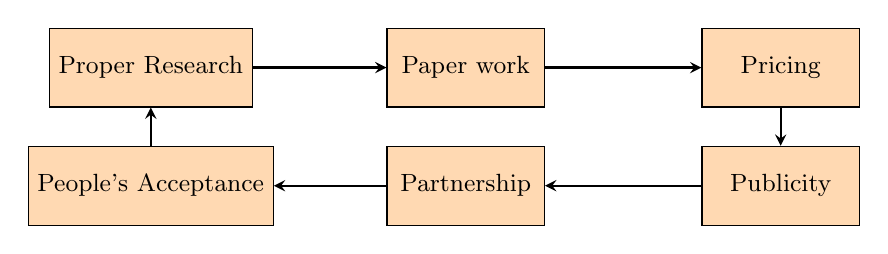
\begin{tikzpicture}[node distance=1.5cm]

\node(p0)[process]{\small Proper Research};
\node(p1)[process, right of=p0, xshift=2.5cm]{\small Paper work};
\node(p2)[process, right of=p1, xshift=2.5cm]{\small Pricing};
\node(p3)[process, below of=p2]{\small Publicity};
\node(p4)[process, below of=p1]{\small Partnership};
\node(p5)[process, below of=p0]{\small People's Acceptance};

\draw[arrow](p0)--(p1);
\draw[arrow](p1)--(p2);
\draw[arrow](p2)--(p3);
\draw[arrow](p3)--(p4);
\draw[arrow](p4)--(p5);
\draw[arrow](p5)--(p0);

\end{tikzpicture}
\end{frame}
